\section{Semana 5 e 6 - Design Point+Wing\&Tail+Engine Selection}
\subsection{Introdução}
Esta secção apresenta os desenvolvimentos durante as semanas 5 e 6. Dada a falta duma reunião de acompanhamento na semana 5, devido a \textbf{??friado or something??}, o trabalho foi realizado continuamente ao longo destas duas semanas, sendo, por isso, amalgamadas numa única secção.\par
O Design Point foi o principal aspeto desenvolvido ao longo dessas duas semanas, sendo um trabalho contínuo. FOi conseguido um desgin satisfatório\par
A seleção da Wing\&Tail foi realizado por \textbf{inserir numero de membros} membros da equipa, sendo mais desenvolvido na semana 6. Foi conseguido um resultado satisfatório, mas os cálculos de desempempenho realizados pelo programa não ficaram ainda corrigidos totalmente para a escolha. Foi considerada uma estimativa conservadora.\par
O Engine Selection benefeciou do nosso estudo de mercado anterior e da tabela fornecido por o docente de motores disponiveis no mercado, tendo ocupado pouco tempo e obtido um resultado satisfatório.\par

\subsection{Desgin Point}
O Design Point foi novamente desenvolvido esta semana, revelando-se um trabalho moroso e demorado, tendo parte da equipa trabalhado exclusivamente neste, a fim de distribuir melhor o trabalho. O desenvolvimento foi feito por turnos, principal e inicialmente, a fim de cada um atacar o problema de ângulos diferentes. Este trabalho consistiu principalmente em ajustar os seguintes valores:
\begin{itemize}
    \item Wing Aspect Ratio
    \item Components Mass
    \item Mission Segment Range - principalmente o Cruise Range
    \item Mission Segment Velocity
    \item Mission Segment Altitude
\end{itemize}
Após trabalho individual, continuamente comunicado e partilhado com o resto do grupo, foi desenvolvido trabalho em conjunto a fim de partilhar e melhor afinar os ajustes, bem como detetar problemas adicionais.\par
No início da \textbf{sexta ou quinta semana?? acho que sexta}, segunda-feira, por análise do ficheiro adt.m, foi descoberto que existia um segundo parâmetro adicional, que podia ser chamado que fazia o programa escrever todos os resultados obtidos, bem como os hardcoded, num ficheiro json. Ao correr o programa com este parâmetro, um erro foi gerado no terminal, indicando que o ficheiro json não consegui ser gerado devido a tentar escrever um formato não suportado. Não era indicado pela mensagem, no entanto, que o que o impedia em concreto era a existência de um número complexo num dos dados. Por inspeção direta das variáveis geradas pelo programa, foi descoberto, que a massa da bateria e a massa do combustível eram imaginárias e que tal seria provavelmente a razão pela qual o json não era gerado. Foi teorizado, e dois dias depois confirmado pelos developers do programa, que a massa imaginária implicava que o avião não conseguia realizar o trajeto proposto. Concretamente, uma das mass fractions seria maior que um, o que revela um cenário impossível. Tal levou ao range ter que ser diminuído para cerca de 33km por cruise segment, havendo 3 no total, e impeliu uma procura por valores errados nas definições, dado que este range extremamente curto não era realista. Como termo de comparação de alcance, foi utilizado o AW 139, que tem um alcance máximo de 1032km.\par
Nessa mesma semana, quinta-feira, foi teorizado que o brake-specific fuel consumption estava errado, dado que era um dos valores default ainda não alterados e o único que não os das asas que nos parecesse alterar o consumo de combustível. Baseado em \textbf{{\Large Inserir citação que agr não sei onde está}}, concluímos que estava errado por duas ordens grandeza, o que indicaria que ou foi mal copiado ou estava escrito em unidades diferentes das SI. Após falar com um dos programadores do programa disponibilizado, concluiu-se que esse valor estava em unidades imperiais, apesar dos outros valores default estarem em SI, estando errada por duas ordens de grandeza.\par
Ao procurar corrigir valores antes de se mudar o brake specific fuel consumption, tentou-se conseguir o alcance máximo possível. Foi descoberto que valores perto de 35km para os três segmentos de cruise realizavam um perfil de missão possível. Ao ajustar o aspect ratio, conseguia-se alterar o valor máximo, mas sem ultrapassar muito este valor, situando-se no máximo a 40km. Escolheu-se optimizar, então, os cruise segments individualmente. Ao realizar tal, foi descoberto que o programa permitia ter um alcance infinito no último segmento de cruise, ou seja, no de retorno ao hospital. Era previsto, pelo programa, que seria possível voar na ordem milhões de kilometros, estimando um combustível necessário de 25kg. Após falar com um dos programadores, na mesma reunião que a suprareferida, foi concluído que havia um bug, consistindo em um das equações de desempenho estar a ser mal realizada. Foi-nos disponibilizada a versão sem erros, posteriormente.\par
É apresentado em baixo o gráfico do melhor design point obtido.
\FloatBarrier
\begin{figure}[h]
    \centering
    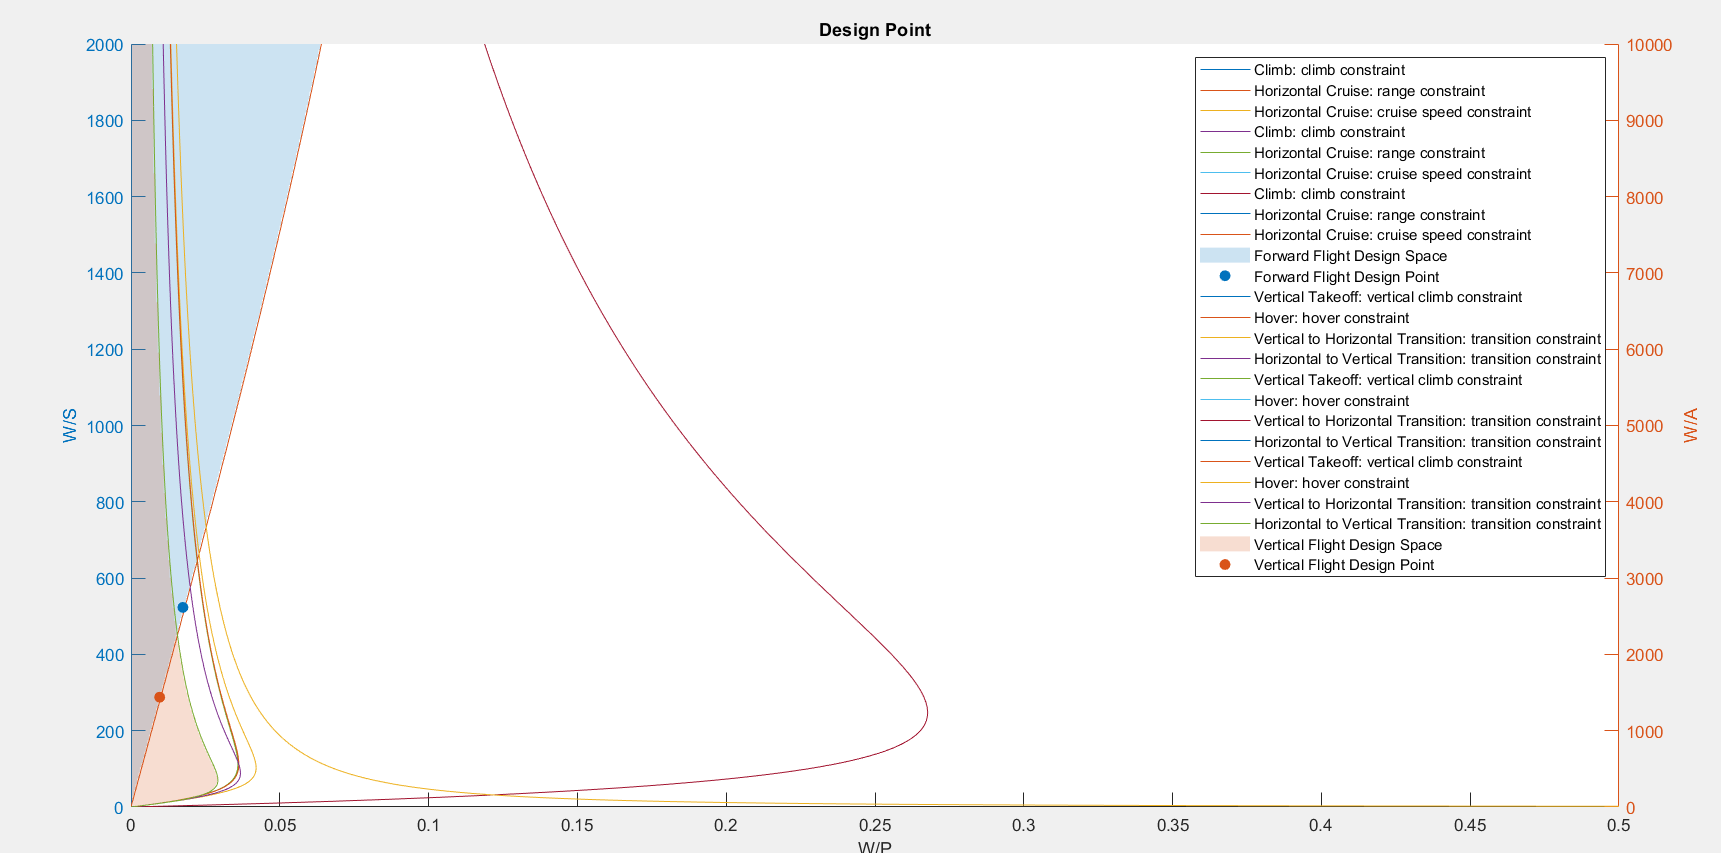
\includegraphics[width=\textwidth]{Imagens/semana6_com_brake_specific_incorreto_designpoint.PNG}
    \caption{Desgin Point com brake-specific fuel consumption incorreto e cerca de 35 km em cada cruise segment - Semana 6}
    \label{designpoint_plot_semana6_correto_specifc_fuel consumption}
\end{figure}
\FloatBarrier

Em baixo, é apresentada a tabela \ref{"tabela_wrong_fuel_consumption"}, onde se encontram os valores para a missão descrita no último design. Note-se os valores do alcance nos segmentos de cruise, uma menor altitude de cruise, bem como valores baixos para altitudes, velocidades e tempos nos outros segmentos em geral. Tal evidência as restrições que nos levaram a acreditar que um dos valores default haveria de estar errado.\par
\FloatBarrier 
 \begin{table}[h] 
 \begin{adjustbox}{width=1\textwidth} 
 \begin{tabular}{|c|c|c|}
 \hline 

\makecell{name: Taxi at Hospital ; \\ type: taxi ; \\ energy\_network: Hybrid Energy Network ; \\ time: 120 ; \\ altitude: 0 ; \\ } & \makecell{name: Vertical Takeoff ; \\ type: vertical\_climb ; \\ energy\_network: Electric Energy Network @ vertical flight ; \\ velocity: 3.5 ; \\ altitude: [0, 50] ; \\ } & \makecell{name: Hover ; \\ type: hover ; \\ energy\_network: Electric Energy Network @ vertical flight ; \\ altitude: 50.0 ; \\ time: 5 ; \\ }\\ \hline \\ 
\makecell{name: Vertical to Horizontal Transition ; \\ type: transition ; \\ energy\_network: Hybrid Energy Network ; \\ altitude: 50 ; \\ transition\_angle: 90 ; \\ time: 12 ; \\ velocity: [0, 16] ; \\ } & \makecell{name: Climb ; \\ type: climb ; \\ energy\_network: Hybrid Energy Network ; \\ velocity: 16 ; \\ altitude: [50, 2500] ; \\ angle: 7.2 ; \\ } & \makecell{name: Horizontal Cruise ; \\ type: cruise ; \\ energy\_network: Hybrid Energy Network @Cruise ; \\ velocity: 97 ; \\ range: 35000 ; \\ altitude: 2500 ; \\ }\\ \hline \\ 
\makecell{name: Approach ; \\ type: descent ; \\ energy\_network: Hybrid Energy Network ; \\ velocity: -20 ; \\ altitude: [2500, 50] ; \\ angle: -7 ; \\ } & \makecell{name: Horizontal to Vertical Transition ; \\ type: transition ; \\ energy\_network: Hybrid Energy Network ; \\ altitude: 50 ; \\ transition\_angle: 40 ; \\ time: 12 ; \\ velocity: [20, 0] ; \\ } & \makecell{name: Vertical Landing at Site ; \\ type: vertical\_descent ; \\ energy\_network: Electric Energy Network @ vertical flight ; \\ velocity: -4 ; \\ altitude: [50, 0] ; \\ }\\ \hline \\ 
\makecell{name: Passenger Tending For Pickup ; \\ type: landing ; \\ energy\_network: Hybrid Energy Network ; \\ time: 1800 ; \\ altitude: 0 ; \\ } & \makecell{name: Passenger Collection ; \\ type: load\_step ; \\ mass: 100 ; \\ time: 0 ; \\ altitude: 0 ; \\ } & \makecell{name: Vertical Takeoff ; \\ type: vertical\_climb ; \\ energy\_network: Electric Energy Network @ vertical flight ; \\ velocity: 4 ; \\ altitude: [0, 50] ; \\ }\\ \hline \\ 
\makecell{name: Hover ; \\ type: hover ; \\ energy\_network: Electric Energy Network @ vertical flight ; \\ altitude: 50.0 ; \\ time: 5 ; \\ } & \makecell{name: Vertical to Horizontal Transition ; \\ type: transition ; \\ energy\_network: Hybrid Energy Network ; \\ altitude: 50 ; \\ transition\_angle: 60 ; \\ time: 12 ; \\ velocity: [0, 16] ; \\ } & \makecell{name: Climb ; \\ type: climb ; \\ energy\_network: Hybrid Energy Network ; \\ velocity: 16 ; \\ altitude: [50, 2500] ; \\ angle: 7.2 ; \\ }\\ \hline \\ 
\makecell{name: Horizontal Cruise ; \\ type: cruise ; \\ energy\_network: Hybrid Energy Network @Cruise ; \\ velocity: 97 ; \\ range: 150000 ; \\ altitude: 2500 ; \\ } & \makecell{name: Approach ; \\ type: descent ; \\ energy\_network: Hybrid Energy Network ; \\ velocity: -20 ; \\ altitude: [2500, 50] ; \\ angle: -7 ; \\ } & \makecell{name: Horizontal to Vertical Transition ; \\ type: transition ; \\ energy\_network: Hybrid Energy Network ; \\ altitude: 50 ; \\ transition\_angle: 40 ; \\ time: 12 ; \\ velocity: [20, 0] ; \\ }\\ \hline \\ 
\makecell{name: Vertical Landing at Hospital ; \\ type: vertical\_descent ; \\ energy\_network: Electric Energy Network @ vertical flight ; \\ velocity: -4 ; \\ altitude: [50, 0] ; \\ } & \makecell{name: Passenger Tending For Unloading ; \\ type: landing ; \\ energy\_network: Hybrid Energy Network ; \\ time: 550 ; \\ altitude: 0 ; \\ } & \makecell{name: Passenger Unloading Step ; \\ type: load\_step ; \\ mass: -100 ; \\ time: 0 ; \\ altitude: 0 ; \\ }\\ \hline \\ 
\makecell{name: Vertical Takeoff ; \\ type: vertical\_climb ; \\ energy\_network: Electric Energy Network @ vertical flight ; \\ velocity: 3.5 ; \\ altitude: [0, 50] ; \\ } & \makecell{name: Hover ; \\ type: hover ; \\ energy\_network: Electric Energy Network @ vertical flight ; \\ altitude: 50.0 ; \\ time: 5 ; \\ } & \makecell{name: Vertical to Horizontal Transition ; \\ type: transition ; \\ energy\_network: Hybrid Energy Network ; \\ altitude: 50 ; \\ transition\_angle: 60 ; \\ time: 12 ; \\ velocity: [0, 16] ; \\ }\\ \hline \\ 
\makecell{name: Climb ; \\ type: climb ; \\ energy\_network: Hybrid Energy Network ; \\ velocity: 16 ; \\ altitude: [50, 2500] ; \\ angle: 7.2 ; \\ } & \makecell{name: Horizontal Cruise ; \\ type: cruise ; \\ energy\_network: Hybrid Energy Network @Cruise ; \\ velocity: 97 ; \\ range: 999999999999999100000 ; \\ altitude: 2500 ; \\ } & \makecell{name: Approach ; \\ type: descent ; \\ energy\_network: Hybrid Energy Network ; \\ velocity: -20 ; \\ altitude: [2500, 50] ; \\ angle: -7 ; \\ }\\ \hline \\ 
\makecell{name: Horizontal to Vertical Transition ; \\ type: transition ; \\ energy\_network: Hybrid Energy Network ; \\ altitude: 50 ; \\ transition\_angle: 40 ; \\ time: 12 ; \\ velocity: [20, 0] ; \\ } & \makecell{name: Vertical Landing at Base ; \\ type: vertical\_descent ; \\ energy\_network: Electric Energy Network @ vertical flight ; \\ velocity: -4 ; \\ altitude: [50, 0] ; \\ } & \makecell{name: Final Post Landing Checkups ; \\ type: landing ; \\ energy\_network: Hybrid Energy Network ; \\ time: 120 ; \\ altitude: 0 ; \\ }\\ \hline \\ 
\end{tabular} 

 \caption{Caracterização dos segmentos de missão - semana 6, primeiro design com brake specific fuel consumption correto} \label{"tabela_wrong_fuel_consumption"}
 \end{adjustbox}
 \end{table} 
 \FloatBarrier 

Após corrigir o brake-specific fuel consumption, e ajustar o range para 200km por segmento de cruise, ficando com um alcance superior a 700km (600km de cruise + 100+ km de subida e descida na diagonal), obteve-se os seguintes resultados:
\FloatBarrier
\begin{figure}[h]
    \centering
    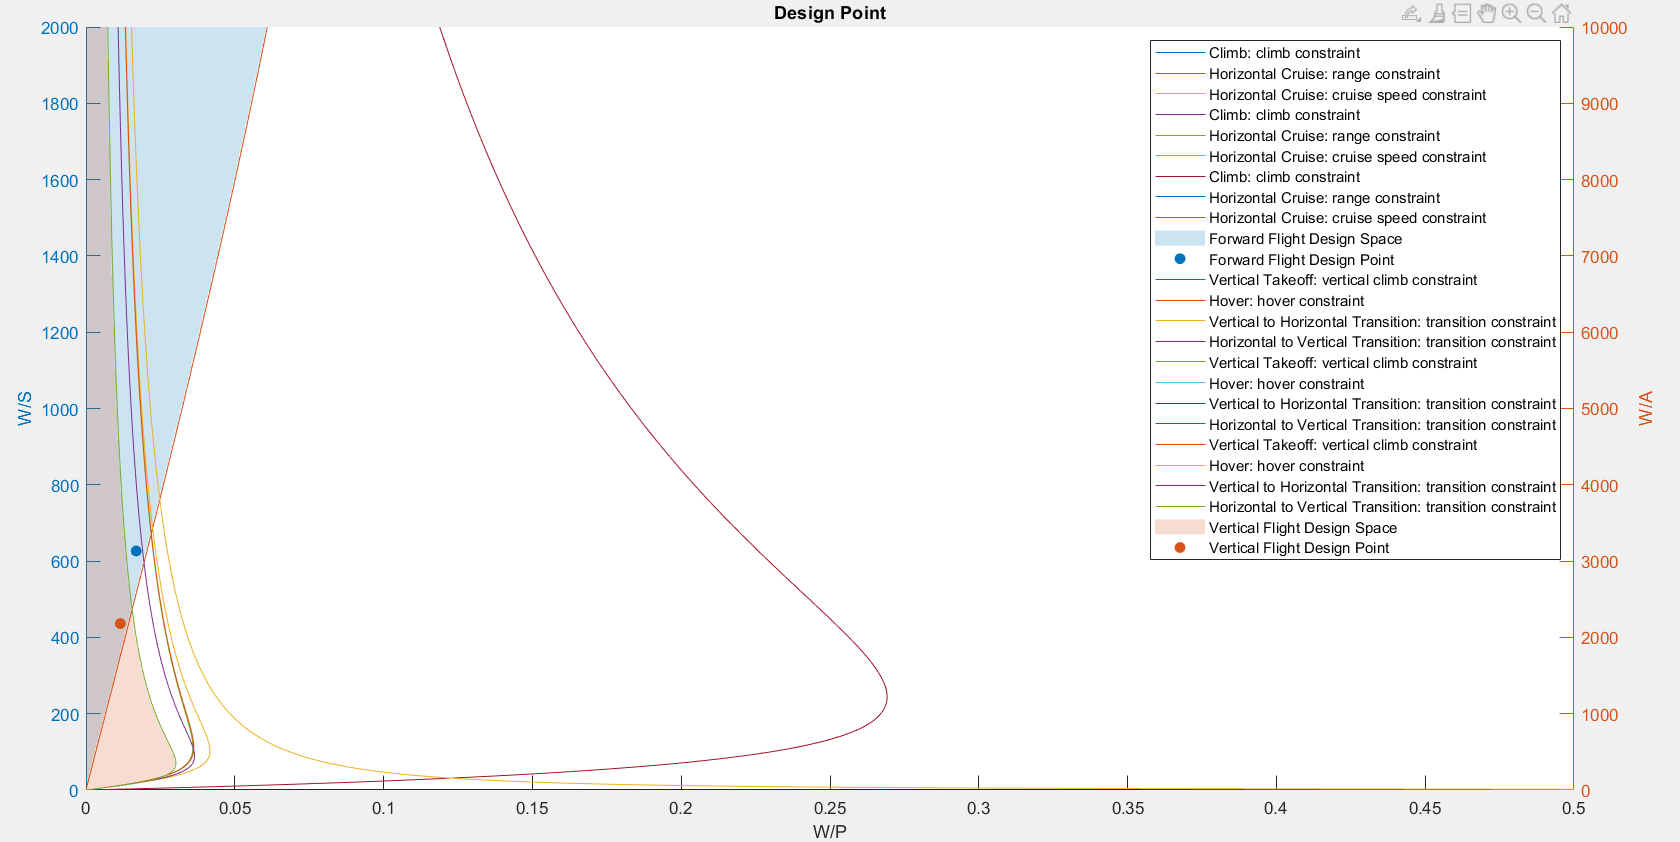
\includegraphics[width=\textwidth]{Imagens/semana6_com_brake_specific_correto_designpoint.PNG}
    \caption{Desgin Point com brake-specific fuel consumption ajustado e 700+ km de alcance- Semana 6}
    \label{designpoint_plot_semana6_correto_specifc_fuel consumption}
\end{figure}
\FloatBarrier

\section{Wing\&Tail}
\section{Engine Selection}